\documentclass[10pt]{beamer}
\usetheme[
%%% option passed to the outer theme
%    progressstyle=fixedCircCnt,   % fixedCircCnt, movingCircCnt (moving is deault)
  ]{Berlin}
  
% If you want to change the colors of the various elements in the theme, edit and uncomment the following lines

% Change the bar colors:
%\setbeamercolor{Feather}{fg=red!20,bg=red}

% Change the color of the structural elements:
%\setbeamercolor{structure}{fg=red}

% Change the frame title text color:
%\setbeamercolor{frametitle}{fg=blue}

% Change the normal text color background:
%\setbeamercolor{normal text}{fg=black,bg=gray!10}

%-------------------------------------------------------
% INCLUDE PACKAGES
%-------------------------------------------------------

\usepackage[utf8]{inputenc}
\usepackage[english]{babel}
\usepackage[T1]{fontenc}
\usepackage{amsmath}
\usepackage{helvet}
\usepackage{multirow}
\usepackage{graphicx}
\usepackage{comment}
\usepackage[absolute,overlay]{textpos}
\usepackage[pdf]{pstricks}
\usepackage{pst-node}
\usepackage{tikz}
\usetikzlibrary{arrows,automata,positioning}
\usetikzlibrary{shapes.multipart}
\usetikzlibrary{decorations.markings}
\usetikzlibrary{decorations.pathreplacing}

%-------------------------------------------------------
% DEFFINING AND REDEFINING COMMANDS
%-------------------------------------------------------

% colored hyperlinks
%\renewcommand*{\Footnotemark}[1]{\NCC@makefnmark{#1}}
\newcommand{\chref}[2]{
  \href{#1}{{\usebeamercolor[bg]{Feather}#2}}
}
\newcommand{\tuple}[1]{{\langle #1 \rangle}}
\newcommand{\pre}{\mathsf{pre}}     % precondition
\newcommand{\eff}{\mathsf{eff}}     % effect
\newcommand{\cond}{\mathsf{cond}}   % conditional effect

\newcommand{\X}{\mathcal{X}}
\newcommand{\F}{\mathcal{F}}
\newcommand{\A}{\mathcal{A}}
\newcommand{\N}{\mathcal{N}}
\newcommand{\I}{\mathcal{I}}
\newcommand{\real}{\mathbb{R}}
\newcommand{\Dw}{\mathcal{D}}
\newcommand{\Xw}{\mathcal{X}}
\newcommand{\Aw}{\mathcal{A}}
\newcommand{\Rw}{\mathcal{R}}
\newcommand{\OO}{\mathcal{O}}
\newcommand{\tOO}{\wt{\OO}}
\newcommand{\II}[1]{\mathbb{I}{\left\{#1\right\}}}
\newcommand{\PP}[1]{\mathbb{P}\left[#1\right]}
\newcommand{\EE}[1]{\mathbb{E}\left[#1\right]}
\newcommand{\EEs}[2]{\mathbb{E}_{#2}\left[#1\right]}
\newcommand{\PPt}[1]{\mathbb{P}_t\left[#1\right]}
\newcommand{\EEt}[1]{\mathbb{E}_t\left[#1\right]}
\newcommand{\PPi}[1]{\mathbb{P}_i\left[#1\right]}
\newcommand{\EEi}[1]{\mathbb{E}_i\left[#1\right]}
\newcommand{\EEp}[1]{\mathbb{E}_{\pi,P}\left[#1\right]}
\newcommand{\EEcp}[2]{\mathbb{E}_{\pi,P}\left[\left.#1\right|#2\right]}
\newcommand{\PPc}[2]{\mathbb{P}\left[#1\left|#2\right.\right]}
\newcommand{\PPct}[2]{\mathbb{P}_t\left[#1\left|#2\right.\right]}
\newcommand{\PPcc}[2]{\mathbb{P}\left[\left.#1\right|#2\right]}
\newcommand{\PPcct}[2]{\mathbb{P}_t\left[\left.#1\right|#2\right]}
\newcommand{\PPcci}[2]{\mathbb{P}_i\left[\left.#1\right|#2\right]}
\newcommand{\EEc}[2]{\mathbb{E}\left[#1\left|#2\right.\right]}
\newcommand{\EEcc}[2]{\mathbb{E}\left[\left.#1\right|#2\right]}
\newcommand{\EEcs}[3]{\mathbb{E}_{#3}\left[\left.#1\right|#2\right]}
\newcommand{\EEcct}[2]{\mathbb{E}_t\left[\left.#1\right|#2\right]}
\newcommand{\EEcci}[2]{\mathbb{E}_i\left[\left.#1\right|#2\right]}
\renewcommand{\th}{\ensuremath{^{\mathrm{th}}}}
\def\argmin{\mathop{\mbox{ arg\,min}}}
\def\argmax{\mathop{\mbox{ arg\,max}}}
\newcommand{\ra}{\rightarrow}

\newcommand{\norm}[1]{\left\|#1\right\|}
\newcommand{\onenorm}[1]{\norm{#1}_1}
\newcommand{\infnorm}[1]{\norm{#1}_\infty}
\newcommand{\iprod}[2]{\left\langle#1,#2\right\rangle}
\newcommand{\ev}[1]{\left\{#1\right\}}
\newcommand{\pa}[1]{\left(#1\right)}
\newcommand{\bpa}[1]{\bigl(#1\bigr)}
\newcommand{\Bpa}[1]{\Bigl(#1\Bigr)}
\newcommand{\sign}{\mbox{sign}}
\newcommand{\wh}{\widehat}
\newcommand{\wt}{\widetilde}
\newcommand{\transpose}{^\top}

\newcommand{\loss}{\ell}
\newcommand{\hloss}{\wh{\loss}}
\newcommand{\hL}{\wh{L}}
\newcommand{\tZ}{\wt{Z}}
\newcommand{\reg}{\mathfrak{R}}
\newcommand{\hreg}{\widehat{\reg}}
\newcommand{\hr}{\wh{r}}
\newcommand{\hv}{\wh{v}}
\newcommand{\hq}{\wh{q}}
\newcommand{\hmu}{\wh{\mu}}
\newcommand{\hR}{\wh{R}}
\newcommand{\tmu}{\wt{\mu}}
\newcommand{\tN}{\wt{N}}
\newcommand{\RE}[2]{\mbox{RE}\left(\left.#1\right\|#2\right)}
\newcommand{\KL}[2]{\mbox{KL}\left(#1\middle\lVert#2\right)}
\newcommand{\DD}[3]{D_{#3}\left(#1\middle\lVert#2\right)}
\newcommand{\DDC}[2]{\DD{#1}{#2}{C}}
\newcommand{\DDS}[2]{\DD{#1}{#2}{S}}

\newcommand{\trho}{\wt{\rho}}

\definecolor{gold}{rgb}{1,0.75,0}
\definecolor{darkred}{rgb}{0.75,0,0}
\setbeamercolor*{goldc}{fg=black,bg=gold}
\definecolor{darkpurp}{rgb}{0.4,0.2,0.4}
\setbeamercolor*{purpc}{fg=white,bg=darkpurp}
\setbeamercolor*{redc}{fg=white,bg=darkred}
\newcommand{\hG}[1]{\large \textcolor{darkred}{#1}}

\newcommand{\redd}[1]{\textcolor{darkred}{#1}}
\newcommand{\goldd}[1]{\textcolor{gold}{#1}}

\definecolor{ballblue}{rgb}{0.0, 0.53, 0.74}
\definecolor{lightgray}{rgb}{0.85, 0.85, 0.85}

%-------------------------------------------------------
% INFORMATION IN THE TITLE PAGE
%-------------------------------------------------------

\title[] % [] is optional - is placed on the bottom of the sidebar on every slide
{ % is placed on the title page
      \textbf{Machine Learning}
}

\author[Jonsson \& G\'omez]
{      Anders Jonsson \& Vicen\c{c} G\'omez \\
\vspace*{0.5cm}
Master in Intelligence Interactive Systems\\
2021-22\\
\vspace*{0.5cm}
Lecture 5\\
Common algorithms for supervised learning
%      {\ttfamily bagchi.bhaskar@cse.iitkgp.ernet.in}
}

\date{}

\AtBeginSection[]
{
   \begin{frame}
       \frametitle{Content}
       \tableofcontents[currentsection]
   \end{frame}
}

%-------------------------------------------------------
% THE BODY OF THE PRESENTATION
%-------------------------------------------------------

\begin{document}

%-------------------------------------------------------
% THE TITLEPAGE
%-------------------------------------------------------

\begin{frame}[plain,noframenumbering] % the plain option removes the header from the title page, noframenumbering removes the numbering of this frame only
  \titlepage % call the title page information from above
\end{frame}

\begin{frame}{Content}{}
\tableofcontents
\end{frame}

\section{Decision Trees}

\begin{frame}
  \frametitle{Definition}
  \begin{itemize}
    \item Wikipedia: ``A {\color{red} decision tree} is a decision {\color{blue} support tool} that uses a {\color{green} tree-like model of decisions} and their possible consequences, including {\color{purple} chance event outcomes, resource costs, and utility}''
  \end{itemize}
\end{frame}

\begin{frame}
  \frametitle{Example}
  \begin{center}
  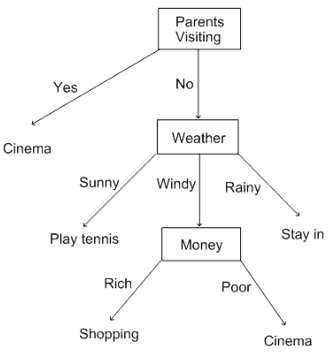
\includegraphics[height=6cm]{images/tree.png}
  \end{center}
\end{frame}

\begin{frame}
  \frametitle{Components}
  \begin{itemize}
    \item {\color{red} Internal node}: represents a \underline{test} on a given feature
	\item {\color{blue} Branch}: represents a possible \underline{outcome} of a given test
	\item {\color{green} Leaf node}: represents a \underline{label} or \underline{decision} 
  \end{itemize}
\end{frame}

\begin{frame}
  \frametitle{Advantages}
  \begin{itemize}
    \item Easy to understand and interpret!
	\item Useful even when little data is available
	\item Allow experts to express knowledge about a given problem
	\item Relatively easy to extend with additional scenarios
  \end{itemize}
\end{frame}

\begin{frame}
  \frametitle{Applications}
  \begin{itemize}
    \item {\color{red} Operations research}: help identify solutions to complex decision-making problems
    \item {\color{blue} Management}: tool for making strategic business decisions
	\item {\color{green} Medicine}: decide on a treatment for a given set of symptoms
  \end{itemize}
\end{frame}

\begin{frame}
  \frametitle{Relationship to Machine Learning}
  \begin{itemize}
	\item A decision tree can represent a hypothesis $h(x)$!
	\item {\color{red} Input set} $\mathcal{X} = \mathcal{X}^1\times\cdots\times\mathcal{X}^d$
    \item {\color{blue} Input} $x\in \mathcal{X}$: vector of feature values
	\item {\color{green} Output}: Label $h(x)$ on the leaf node reached by resolving the
		test at each internal node
  \end{itemize}
\end{frame}

\begin{frame}
  \frametitle{Example}
  \begin{itemize}
	\item {\color{red} Input set} $\mathcal{X} = \mathcal{X}^1\times\mathcal{X}^2\times\mathcal{X}^3$

	\vspace*{.3cm}

	\begin{tabular}{ll}
	$\mathcal{X}^1 = \{$Yes, No$\}$ & (parents visiting)\\
	$\mathcal{X}^2 = \{$Sunny, Windy, Rainy$\}$ & (weather)\\
	$\mathcal{X}^3 = \{$Rich, Poor$\}$ & (money)
	\end{tabular}

	\vspace*{.3cm}

	\item {\color{blue} Target set}: $\mathcal{Y}=\{$Cinema, Play tennis, Shopping, Stay in$\}$
	\item {\color{green} Example input}: $x=($No, Windy, Poor$)\in \mathcal{X}$
  \end{itemize}
\end{frame}

\begin{frame}
  \frametitle{Example}
  \begin{center}
  \begin{tikzpicture}[overlay]
	\node at (0,0) {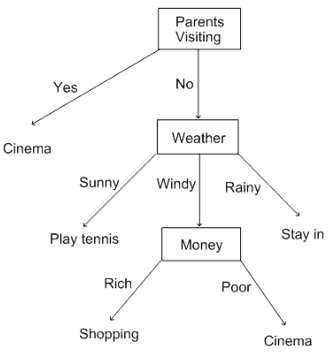
\includegraphics[height=6cm]{images/tree.png}};
    \put(-4.5,61.6){\tikz \draw[red,thick] (0,0) rectangle (1.375,0.675);}
    \put(-4.5,11.6){\tikz \draw[red,thick] (0,0) rectangle (1.35,0.575);}
    \put(-2.5,-40.4){\tikz \draw[red,thick] (0,0) rectangle (1.3,0.575);}
    \put(15.0,28){\tikz \draw[red,thick,<-] (0,0) --(0,1.2);}
    \put(15.5,-24){\tikz \draw[red,thick,<-] (0,0) --(0,1.225);}
    \put(35.5,-72){\tikz \draw[red,thick,<-] (.75,0) --(0,1.125);}
    \put(43,-85.5){\tikz \draw[blue,thick,rounded corners] (0,0) rectangle (1.025,0.475);}
  \end{tikzpicture}
  \end{center}
\end{frame}

\begin{frame}
  \frametitle{Input set}
  \begin{center}
  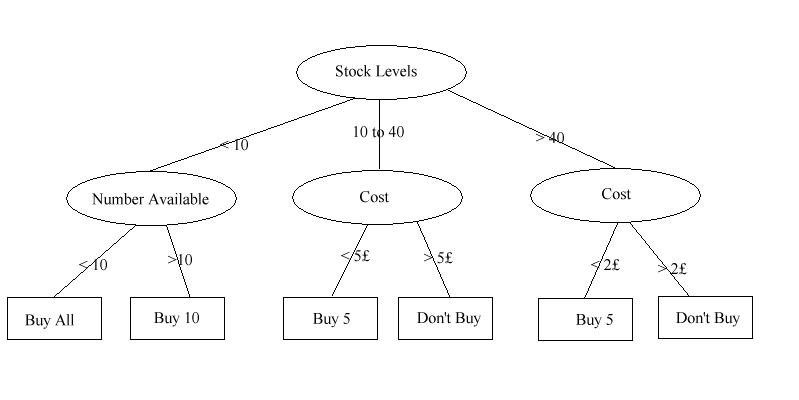
\includegraphics[height=5cm]{images/dtree.png}
  \end{center}
  \begin{itemize}
    \item {\color{red} Finite set}: test outcome is a specific value
	\item {\color{green} Real numbers}: test outcome is an interval
  \end{itemize}
\end{frame}

\begin{frame}
  \frametitle{Algorithms}
  \begin{itemize}
    \item ID3 (Iterative Dichotomiser 3)
    \item {\color{red} C4.5} (successor of ID3)
    \item CART (Classification And Regression Tree)
    \item CHAID (CHi-squared Automatic Interaction Detector)
    \item MARS: (Multivariate Adaptive Regression Splines)
  \end{itemize}
\end{frame}

\begin{frame}
  \frametitle{Entropy}
  \begin{itemize}
    \item Measures {\color{red} information content}
    \item Large entropy $\Rightarrow$ unpredictable outcome
	\item For a random variable $X$, the entropy is expressed as
	\[H(X)=\mathbb{E}[I(X)]=\mathbb{E}[-\log(P(X))]\]
  \begin{itemize}
	\item $I(X)$: information content of $X$ (itself a random variable)
	\item $P(X)$: probability mass function
  \end{itemize}
	\item {\color{red} Unsupervised} training set $S=(x_1,\ldots,x_m)$: \[H(S)=-\sum_{i=1}^mP(x_i)\log P(x_i)\]
  \end{itemize}
\end{frame}

\begin{frame}
  \frametitle{Entropy of input-label pairs}
  \begin{itemize}
    \item Training set $S=((x_1,y_1),\ldots,(x_m,y_m))$ of input-label pairs
	\item For each $y\in\mathcal{Y}$, {\color{red} $S(\mathcal{Y},y)\equiv\{(x_i,y_i)\in S:y_i=y\}\subseteq S$}
	\item For each $y\in\mathcal{Y}$, {\color{blue} $P(y)\equiv\frac{|S(\mathcal{Y},y)|}{|S|}$}
	\item Entropy {\color{green} $H(S)=-\sum_{y\in \mathcal{Y}}P(y)\log P(y)$}
  \end{itemize}
\end{frame}

\begin{frame}
  \frametitle{Information gain}
  \begin{itemize}
    \item Expected information gain $=$ {\color{red} change} in entropy
    \item $IG(S,\mathcal{X}^i)=H(S)-H(S|\mathcal{X}^i)$
    \item $H(S|\mathcal{X}^i)=\sum_{v\in \mathcal{X}^i}
		\frac{|S(\mathcal{X}^i,v)|}{|S|}H(S(\mathcal{X}^i,v))$
  \end{itemize}
\end{frame}

\begin{frame}
  \frametitle{Learning Decision Trees}
  \begin{itemize}
    \item Start with a single root node
	\item For each feature $\mathcal{X}^i$ not used in tests, compute $IG(S, \mathcal{X}^i)$
	\item Let $\mathcal{X}^*=\arg\max_{\mathcal{X}^i} IG(S, \mathcal{X}^i)$
	\item Split the node on $\mathcal{X}^*$ and distribute data points to new leaves
	\item Repeat at leaves until no more information gain is possible
  \end{itemize}
\end{frame}

\begin{frame}
  \frametitle{Disadvantages}
  \begin{itemize}
	\item {\color{red} Greedy}: can get stuck in local minima
	\item Does not take into account correlation among attributes
    \item {\color{blue} Overfitting}: overly large decision tree
    \item Difficult to apply to real-valued attributes (where to split?)
  \end{itemize}
\end{frame}

\begin{frame}
  \frametitle{Bayesian Information Criterion}
  \begin{itemize}
    \item Criterion for model selection among a finite set of models
    \item Data set $S=((x_1,y_1),\ldots,(x_m,y_m))$ of size $m$
    \item $\theta$: set of parameters (i.e.~labels)
	\item {\color{red} Likelihood function} $\hat{L}=P(S\mid\theta,T)$ where $T$ is the tree
	\item Bayesian Information Criterion: {\color{blue} $BIC=-2\log\hat{L}+|\theta|\log m$}
	\item Splitting on $\mathcal{X}^i$: $-2\log\hat{L}_1-(-2\log\hat{L}_2)=IG(S,\mathcal{X}^i)$
  \end{itemize}
\end{frame}

\begin{frame}
  \frametitle{{\color{red} B}ootstrap {\color{red} Agg}regat{\color{red} ing} (Bagging)}
  \begin{itemize}
    \item Given a training set $S=((x_1,y_1),\ldots,(x_m,y_m))$,
		generate $k$ smaller training sets of size $m'<m$ by {\color{blue} sampling} from $S$
    \item Learn a separate decision tree for each of the $k$ training sets
	\item Aggregate the output of each decision tree
  \begin{itemize}
    \item Regression: average the outputs
	\item Classification: output by voting
  \end{itemize}
  \end{itemize}
\end{frame}

\begin{comment}
\begin{frame}
  \frametitle{Decision Diagram}
  \begin{center}
  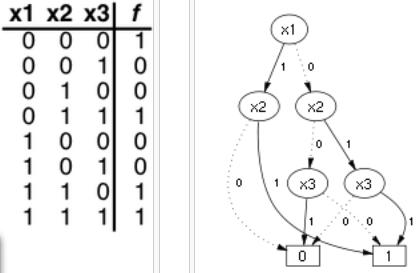
\includegraphics[height=3cm]{images/bdd.jpg}
  \end{center}
  \begin{itemize}
    \item Directed graph rather than tree
    \item More compact than a decision tree
  \end{itemize}
\end{frame}

\begin{frame}
  \frametitle{Ordered Decision Diagram}
  \begin{center}
  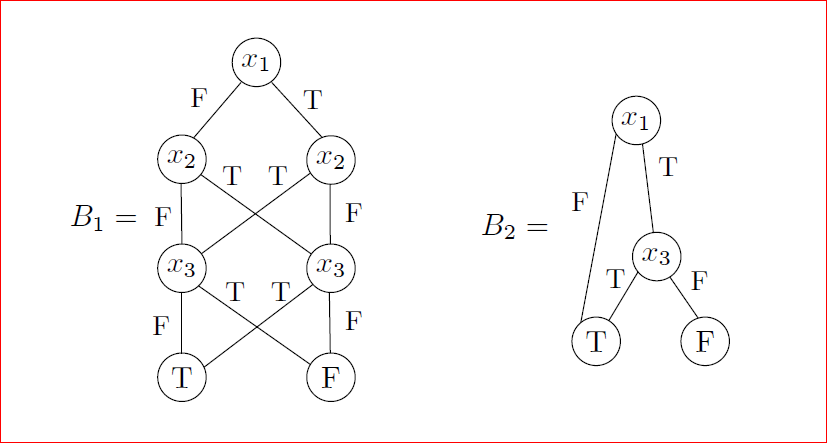
\includegraphics[height=4cm]{images/obdd.png}
  \end{center}
  \begin{itemize}
    \item Fixed feature ordering $x_1,\ldots,x_n$
    \item If $i<j$, tests on $x_i$ always appear {\color{red} above} tests on $x_j$
  \end{itemize}
\end{frame}

\begin{frame}
  \frametitle{Reduced Ordered Decision Diagram}
  \begin{itemize}
    \item Minimal decision diagram representing a given function
	\item {\color{red} Unique} for a particular function and variable ordering!
	\item Supports efficient algorithms:
  \begin{itemize}
    \item Disjunction (sum) of two decision diagrams
    \item Conjunction (product) of two decision diagrams
    \item Existential abstraction: $\exists x_i: F\equiv F(x_i/0)\vee F(x_i/1)$
	\item Universal abstraction $\forall x_i: F\equiv F(x_i/0)\wedge F(x_i/1)$
  \end{itemize}
  \end{itemize}
\end{frame}

\begin{frame}
  \frametitle{Variable ordering}
  \begin{itemize}
    \item Variable ordering can have huge impact on diagram size
	\item Problem: finding an optimal variable ordering is NP-hard
	\item Even worse, it is NP-hard to find an approximately optimal variable ordering
	\item There exist efficient heuristics for finding good variable orderings
  \end{itemize}
\end{frame}

\begin{frame}
  \frametitle{Representation}
  \begin{itemize}
    \item Usually decision diagrams are stored in hash tables
	\item Each node (internal and external) is an element of the hash table
	\item Allows fast merging of two identical sub-diagrams
	\item Problem: garbage collection (removing obsolete nodes)
  \end{itemize}
\end{frame}

\begin{frame}
  \frametitle{Applications of decision diagrams}
  \begin{itemize}
    \item Operations on sparse matrices
    \item Synthesize electronic circuits
	\item Formal verification (proving the correctness of algorithms)
  \end{itemize}
\end{frame}
\end{comment}

\section{Support Vector Machines}

\begin{frame}
  \frametitle{Support vector machine}
  \begin{itemize}
    \item Model for supervised learning
	\item Basic algorithm: binary linear classification ($\mathcal{Y}=\{-1,+1\}$)
	\item Geometry-based: treats data points as spatial coordinates
	\item Invented by Vladimir Vapnik
  \end{itemize}
\end{frame}

\begin{frame}
  \frametitle{Intuition}
  \begin{itemize}
    \item Usually, data is not linearly separable
	\item Idea: {\color{red} increase} the dimensionality!
	\item Data more likely to be linearly separable in new space
	\item Use {\color{blue} kernels} to avoid computational blowup
  \end{itemize}
\end{frame}

\begin{frame}
  \frametitle{Illustration}
  \centerline{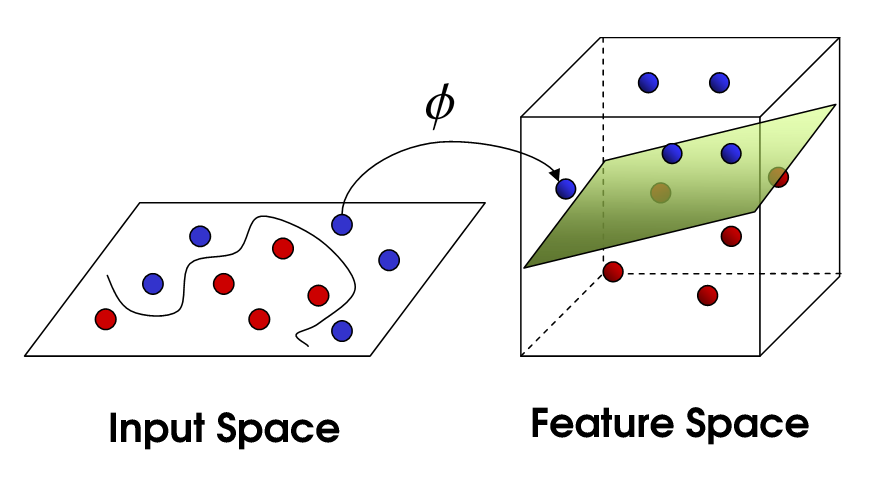
\includegraphics[height=4cm]{images/feature.png}}
\end{frame}

\begin{frame}
  \frametitle{Maximum-margin hyperplane}
  \begin{itemize}
    \item Maximizes the {\color{red} margin}, i.e.~the distance from the data points
    \item Idea: consider {\color{blue} two} boundary hyperplanes
  \end{itemize}
  \vspace{.4cm}
  \centerline{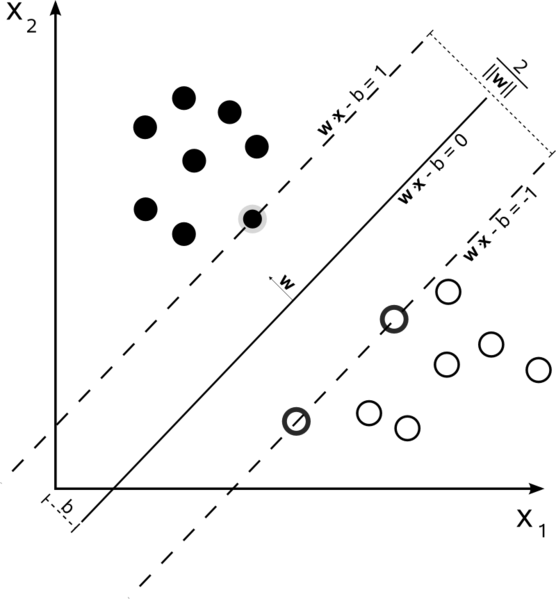
\includegraphics[height=4cm]{images/margin.png}}
\end{frame}

\begin{frame}
  \frametitle{Algorithm}
  \begin{itemize}
    \item Equation of a hyperplane: $\sum_{i=1}^dw_ix_i + b=\langle w,x\rangle+b=0$
    \item {\color{red} Boundary} hyperplanes: $\langle w,x\rangle+b=-1$ and $\langle w,x\rangle+b=1$
    \item Distance between boundary hyperplanes: $2/\|w\|$
	\item Maximize distance $\Rightarrow$ minimize $\|w\|$ $\Rightarrow$ minimize $\frac 1 2 \|w\|^2$
  \end{itemize}
\end{frame}

\begin{frame}
  \frametitle{Constrained optimization}
  \begin{itemize}
    \item Constraints:
  \begin{itemize}
    \item For each $x_i$ such that $y_i=+1$, $\langle w,x_i\rangle+b\geq 1$
    \item For each $x_i$ such that $y_i=-1$, $\langle w,x_i\rangle+b\leq-1$
  \end{itemize}
    \item Rewrite as $y_i(\langle w,x_i\rangle+b)\geq 1$
	\pause
    \item Quadratic programming optimization problem:
  \end{itemize}
	\vspace{.1cm}
  \begin{tabular}{l}
	\vspace{.2cm}
    \hspace*{1cm}$\min_{w,b} \;\; \frac{1}{2}\langle w,w\rangle$\\
	\hspace*{1cm}subject to $y_i(\langle w,x_i\rangle+b)\geq 1$ for each $1\leq i\leq m$
  \end{tabular}
\end{frame}

\begin{frame}
  \frametitle{Support vectors}
  \begin{itemize}
    \item Solution is of the form $w=\sum_{i=1}^m\alpha_iy_ix_i$
	\item {\color{red} Support vectors}: inputs $x_i$ such that $\alpha_i>0$ 
	\item Support vectors satisfy {\color{blue} equality}: $y_i(\langle w,x_i\rangle+b)=1$
  \end{itemize}
\end{frame}

\begin{frame}
  \frametitle{Dual form}
  \begin{itemize}
	\item One can show that the dual optimization problem is defined as
  \end{itemize}
  \begin{tabular}{l}
	\vspace{.2cm}
    \hspace*{1cm}$\max_\alpha \;\; \sum_{i=1}^m\alpha_i-\frac{1}{2}\sum_{i=1}^m\sum_{j=1}^m\alpha_i\alpha_jy_iy_j {\color{red} \langle x_i,x_j\rangle}$\\
	\hspace*{1cm}subject to $\left\{\begin{array}{l}\alpha_i\geq 0\;\mathrm{for}\;\mathrm{each}\;1\leq i\leq m,\\\sum_{i=1}^m\alpha_iy_i=0\end{array}\right.$
  \end{tabular}
\end{frame}

\begin{frame}
  \frametitle{Soft margin}
  \begin{itemize}
    \item Basic algorithm requires data to be linearly separable
	\item {\color{red} Soft margin}: allow mislabelled examples 
	\item Find hyperplane that splits the examples as cleanly as possible
	\item Idea: upper bound each $\alpha_i$ by a constant $C$
	\item Optimization problem not significantly more complex
  \end{itemize}
\end{frame}

\begin{frame}
  \frametitle{Model complexity}
  \begin{itemize}
    \item Vapnik: Model complexity proportional to $\|w\|$
	\item Intuition: if $\|w\|$ is small, the true error of the separating maximum-margin
	hyperplane is close to the training error
	\item Independent of the number of features!
  \end{itemize}
\end{frame}

%\begin{frame}
%  \frametitle{Quadratic programming}
%  \begin{itemize}
%	\item Problem formulation:
%  \end{itemize}
%	\vspace{.2cm}
%  \begin{tabular}{l}
%	\vspace{.2cm}
%    \hspace*{1cm}Minimize $f(x)=\frac{1}{2}x^\top Q x + c^\top x$\\
%	\hspace*{1cm}subject to $\left\{\begin{array}{l}A x\leq b,\\E x= d.\end{array}\right.$
%  \end{tabular}
%	\vspace{.2cm}
%  \begin{itemize}
%	\item $x$, $c$, $b$: vectors of $n$ elements
%    \item $Q$: symmetric $n\times n$ matrix
%  \end{itemize}
%\end{frame}

%\begin{frame}
%  \frametitle{Complexity}
%  \begin{itemize}
%	\item No inequality constraints: problem is linear
%    \item $Q$ {\color{red} positive definite}: $z^\top Q z>0$ for each real, non-zero $z$
%  \begin{itemize}
%	\item $\Rightarrow$ there exists a polynomial-time solution
%  \end{itemize}
%    \item $Q$ has at least one negative eigenvalue: problem is NP-hard
%  \end{itemize}
%\end{frame}

%\begin{frame}
%  \frametitle{Solution techniques}
%  \begin{itemize}
%	\item Interior point algorithms
%	\item Active set algorithm
%	\item Augmented Lagrangian method
%	\item Conjugate gradient method
%	\item Extensions of the simplex algorithm
%  \end{itemize}
%\end{frame}

%\begin{frame}
%  \frametitle{Illustration}
%  \centerline{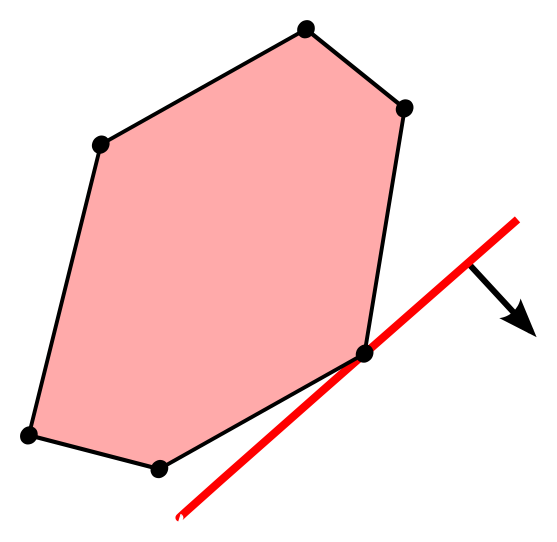
\includegraphics[height=4cm]{images/lp.png}}
%\end{frame}

\begin{frame}
  \frametitle{Non-linear classification}
  \begin{itemize}
    \item Basic algorithm performs binary linear classification
    \item In general, data not linearly separable
    \item Non-linear {\color{red} transformation} from original space to new space
	\item Choose transformation such that data is (almost) linearly separable in transformed space
  \end{itemize}
\end{frame}

\begin{frame}
  \frametitle{Inner product space}
  \begin{itemize}
    \item Vector space that defines an {\color{red} inner product} $\langle\cdot,\cdot\rangle$
	\item Vectors $x$ and $y$ {\color{blue} orthogonal} $\Leftrightarrow$ $\langle x,y\rangle=0$
	\item Inner product induces a {\color{green} norm} $\|x\|=\sqrt{\langle x,x\rangle}$
    \item Generalizes the Euclidean space (inner product $=$ scalar product)
  \end{itemize}
\end{frame}

\begin{frame}
  \frametitle{Kernel trick}
  \begin{itemize}
    \item Map observations from a set $\mathcal{X}$ to an inner product space $V$
	\item {\color{red} Trick}: in $V$, only use algorithms based on inner product
	\item {\color{blue} Kernels} compute inner product directly on elements in $\mathcal{X}$
	\item No need to compute the mapping from $\mathcal{X}$ to $V$ explicitly!
  \end{itemize}
  \begin{tabular}{l}
	\vspace{.2cm}
    \hspace*{1cm}$\max_\alpha \;\; \sum_{i=1}^m\alpha_i-\frac{1}{2}\sum_{i=1}^m\sum_{j=1}^m\alpha_i\alpha_jy_iy_j {\color{red} k(x_i,x_j)}$\\
	\hspace*{1cm}subject to $\left\{\begin{array}{l}\alpha_i\geq 0\;\mathrm{for}\;\mathrm{each}\;1\leq i\leq m,\\\sum_{i=1}^m\alpha_iy_i=0\end{array}\right.$
  \end{tabular}
\end{frame}

\begin{frame}
  \frametitle{Non-linear transformation}
  \begin{itemize}
	\item Map original feature space to high-dimensional space
    \item Find maximum-margin hyperplane in transformed space
	\item Replace each dot product with a {\color{blue} kernel}
		$k(x_1,x_2)=\langle\phi(x_1),\phi(x_2)\rangle$
	\item Use regularization to avoid overfitting
  \end{itemize}
\end{frame}

\begin{frame}
  \frametitle{Common kernels}
  \begin{tabular}{ll}
	$k(x_1,x_2)=x_1^\top x_2$: & dot product (Euclidean)\\
	$k(x_1,x_2)=(x_1^\top x_2)^q$: & polynomial homogeneous\\
	$k(x_1,x_2)=(x_1^\top x_2 + 1)^q$: & polynomial inhomogeneous\\
	$k(x_1,x_2)=\mathrm{exp}(-\gamma\|x_1-x_2\|^2)$: & Gaussian radial basis, $\gamma>0$\\
	$k(x_1,x_2)=\mathrm{tanh}(\kappa x_1^\top x_2 - c)$: & Hyperbolic tangent, $\kappa,c>0$
  \end{tabular}
\end{frame}

\begin{frame}
  \frametitle{Classification}
  \begin{itemize}
	\item Solution in $V$ is of the form $w=\sum_{i=1}^m\alpha_iy_i\phi(x_i)$
	\item {\color{red} Classification} of new example $x$:
	\[\langle w,\phi(x)\rangle=
		\sum_{i=1}^m\alpha_iy_i\langle\phi(x_i),\phi(x)\rangle=
		\sum_{i=1}^m\alpha_iy_ik(x_i,x)\]
	\item In general, there is no $w'$ in $\mathcal{X}$ such that
		$\langle w,\phi(x)\rangle=k(w',x)$
  \end{itemize}
\end{frame}

\begin{frame}
  \frametitle{Intuition of Gaussian radial basis}
  \centerline{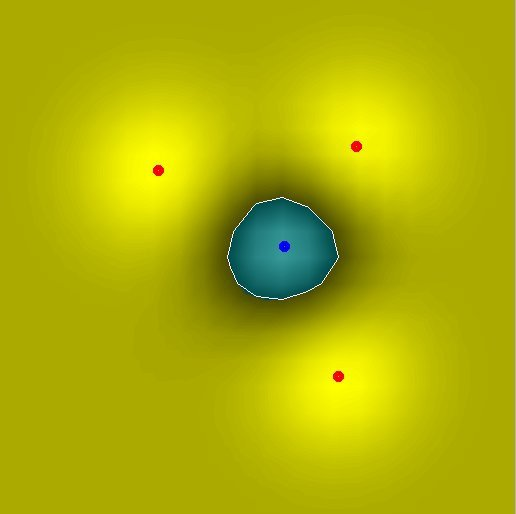
\includegraphics[height=5cm]{images/radial.jpeg}}
\end{frame}

\begin{frame}
  \frametitle{Properties}
  \begin{itemize}
    \item Generalizes the perceptron
	\item Simultaneously minimizes {\color{red} classification error} and maximizes {\color{blue} geometric margin}
	\item Special case of {\color{green} Tikhonov regularizer} $w^{\top}\Gamma^{\top}\Gamma w$
  \end{itemize}
\end{frame}

\begin{frame}
  \frametitle{Disadvantages}
  \begin{itemize}
    \item Highly dependent on the kernel and the kernel parameters
	\item Highly dependent on the soft margin constant $C$
	\item Uncalibrated class membership probabilities
	\item Only directly applicable to two-class tasks
	\item Solved model difficult to interpret
  \end{itemize}
\end{frame}

\begin{frame}
  \frametitle{Common use}
  \begin{itemize}
    \item Use a Gaussian radial basis kernel (single parameter $\gamma$)
	\item {\color{red} Grid search} to find best combination of $\gamma$ and $C$
	\item Use {\color{blue} cross validation} to test each parameter choice
	\item Final model trained on {\color{green} complete} data set using chosen parameters
  \end{itemize}
\end{frame}

\begin{frame}
  \frametitle{Multi-class SVM}
  \begin{itemize}
    \item Generalize the algorithm for binary classification
	\item Classify data with a finite number $L>2$ of class labels
	\item Reduce to multiple binary classification problems
  \end{itemize}
\end{frame}

\begin{frame}
  \frametitle{Multi-class SVM}
  \begin{itemize}
    \item Common approaches:
  \begin{itemize}
    \item OVO: Binary classifier for each label pair, classification by {\color{red} voting}
	\item OVA: Binary classifier for each label with respect to other labels
	\item Directed acyclic graph SVM
  \end{itemize}
	\item There exist approaches that solve a single optimization problem
  \end{itemize}
\end{frame}

\section{Exercises}

\begin{frame}
  \frametitle{Decision tree learning}
  \begin{itemize}
	\item $\mathcal{X} = \mathcal{X}^1 \times \mathcal{X}^2 \times \mathcal{X}^3$ such that $\mathcal{X}^1 = \mathcal{X}^2 = \mathcal{X}^3 = \mathcal{Y} = \{0,1\}$
	\item Each data point is on the format $(x,y) = (x^1,x^2,x^3,y)$
    \item {\color{red} $S=\{(0,0,0,0),(0,1,0,1),(1,0,1,1),(1,1,0,0)\}$}
	\item Apply the algorithm C4.5 to learn a decision tree
  \end{itemize}
\end{frame}

\begin{frame}
  \frametitle{Entropy of $S$}
  \begin{itemize}
    \item {\color{red} $S=\{(0,0,0,0),(0,1,0,1),(1,0,1,1),(1,1,0,0)\}$}
	\item $S(\mathcal{Y},0)=\{(0,0,0,0),(1,1,0,0)\}$, $S(\mathcal{Y},1)=\{(0,1,0,1),(1,0,1,1)\}$
	\pause
	\item $P(0) = \frac {|S(\mathcal{Y},0)|} {|S|} = \frac 2 4 = \frac 1 2$, $P(1) = \frac {|S(\mathcal{Y},1)|} {|S|} = \frac 2 4 = \frac 1 2$
  \end{itemize}
  \pause
  \begin{align*}
	H(S)&=-P(0)\log P(0)-P(1)\log P(1)=\\
	&=-\frac{1}{2}\log\frac{1}{2}-\frac{1}{2}\log\frac{1}{2}=\\
    &=-\log\frac{1}{2}=-(-1)=1
  \end{align*}
\end{frame}

\begin{frame}
  \frametitle{Splitting on $\mathcal{X}^1$}
  \begin{itemize}
    \item {\color{red} $S=\{(0,0,0,0),(0,1,0,1),(1,0,1,1),(1,1,0,0)\}$}
    \item $S_0 = S(\mathcal{X}^1,0)=\{(0,0,0,0),(0,1,0,1)\}$, $S_1 = S(\mathcal{X}^1,1)=\{(1,0,1,1),(1,1,0,0)\}$
	\pause
%	\item $S_0(\mathcal{Y},0)=\{(0,0,0,0)\}$, $S_0(\mathcal{Y},1)=\{(0,1,0,1)\}$, $S_1(\mathcal{Y},0)=\{(1,1,0,0)\}$, $S_1(\mathcal{Y},1)=\{(1,0,1,1)\}$
	\item $P_0(0) = \frac 1 2$, $P_0(1) = \frac 1 2$, $P_1(0) = \frac 1 2$, $P_1(1) = \frac 1 2$
  \end{itemize}
  \pause
  \begin{align*}
	H(S|\mathcal{X}^1)&=\frac{|S_0|}{|S|}H(S_0)+\frac{|S_1|}{|S|}H(S_1)\\
	H(S_0)&=-\frac{1}{2}\log\frac{1}{2}-\frac{1}{2}\log\frac{1}{2}=1\\
	H(S_1)&=-\frac{1}{2}\log\frac{1}{2}-\frac{1}{2}\log\frac{1}{2}=1\\
	IG(S,\mathcal{X}^1)&=H(S)-H(S|\mathcal{X}^1)=1 - \left(\frac 1 2 \cdot 1 + \frac 1 2 \cdot 1 \right) = 0
  \end{align*}
\end{frame}

\begin{frame}
  \frametitle{Splitting on $\mathcal{X}^2$}
  \begin{itemize}
    \item {\color{red} $S=\{(0,0,0,0),(0,1,0,1),(1,0,1,1),(1,1,0,0)\}$}
    \item $S_0 = S(\mathcal{X}^2,0)=\{(0,0,0,0),(1,0,1,1)\}$, $S_1 = S(\mathcal{X}^2,1)=\{(0,1,0,1),(1,1,0,0)\}$
	\pause
%	\item $S_0(\mathcal{Y},0)=\{(0,0,0,0)\}$, $S_0(\mathcal{Y},1)=\{(1,0,1,1)\}$, $S_1(\mathcal{Y},0)=\{(1,1,0,0)\}$, $S_1(\mathcal{Y},1)=\{(0,1,0,1)\}$
	\item $P_0(0) = \frac 1 2$, $P_0(1) = \frac 1 2$, $P_1(0) = \frac 1 2$, $P_1(1) = \frac 1 2$
  \end{itemize}
  \pause
  \begin{align*}
	H(S|\mathcal{X}^2)&=\frac{|S_0|}{|S|}H(S_0)+\frac{|S_1|}{|S|}H(S_1)\\
	H(S_0)&=-\frac{1}{2}\log\frac{1}{2}-\frac{1}{2}\log\frac{1}{2}=1\\
	H(S_1)&=-\frac{1}{2}\log\frac{1}{2}-\frac{1}{2}\log\frac{1}{2}=1\\
	IG(S,\mathcal{X}^2)&=H(S)-H(S|\mathcal{X}^2)=1 - \left(\frac 1 2 \cdot 1 + \frac 1 2 \cdot 1 \right) = 0
  \end{align*}
\end{frame}

\begin{frame}
  \frametitle{Splitting on $\mathcal{X}^3$}
  \begin{itemize}
    \item {\color{red} $S=\{(0,0,0,0),(0,1,0,1),(1,0,1,1),(1,1,0,0)\}$}
    \item $S_0 = S(\mathcal{X}^3,0)=\{(0,0,0,0),(0,1,0,1),(1,1,0,0)\}$, $S_1 = S(\mathcal{X}^3,1)=\{(1,0,1,1)\}$
	\pause
%	\item $S_0(\mathcal{Y},0)=\{(0,0,0,0),(1,1,0,0)\}$, $S_0(\mathcal{Y},1)=\{(0,1,0,1)\}$, $S_1(\mathcal{Y},0)=\emptyset$, $S_1(\mathcal{Y},1)=\{(1,0,1,1)\}$
	\item $P_0(0) = \frac 2 3$, $P_0(1) = \frac 1 3$, $P_1(0) = 0$, $P_1(1) = 1$
  \end{itemize}
  \pause
  \begin{align*}
	H(S|\mathcal{X}^3)&=\frac{|S_0|}{|S|}H(S_0)+\frac{|S_1|}{|S|}H(S_1)\\
	H(S_0)&=-\frac 2 3 \log\frac 2 3 - \frac 1 3 \log\frac 1 3 \approx 0.27\\
	H(S_1)&=-0\log 0- 1\log 1=0\\
	IG(S,\mathcal{X}^3)&=H(S)-H(S|\mathcal{X}^3)=1 - \left(\frac 3 4 \cdot 0.27 + \frac 1 4 \cdot 0 \right) \approx 0.79
  \end{align*}
\end{frame}

\begin{frame}
  \frametitle{Resulting tree}
  \begin{center}
  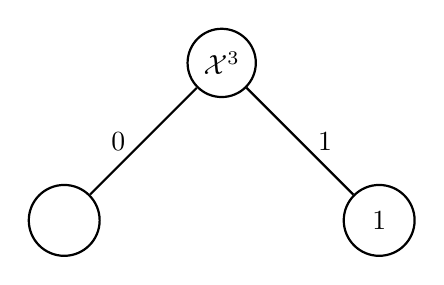
\begin{tikzpicture}
	\node[draw,thick,circle] at (3,3) (a) {$\mathcal{X}^3$};
	\node[draw,thick,circle,minimum size=0.9cm] at (1,1) (b) {};
	\node[draw,thick,circle,minimum size=0.9cm] at (5,1) (c) {$1$};
	\draw[thick] (a) -- (b) node[midway,left,xshift=-.1cm] {$0$};
	\draw[thick] (a) -- (c) node[midway,right,xshift=.1cm] {$1$};
  \end{tikzpicture}
  \end{center}
  \begin{itemize}
    \item Split on left node with $S_0=\{(0,0,0,0),(0,1,0,1),(1,1,0,0)\}$
    \item $S_1=\{(0,1,0,1)\}$ cannot be split any further, so we predict $1$
  \end{itemize}
\end{frame}

\begin{frame}
  \frametitle{Final tree}
  \begin{center}
  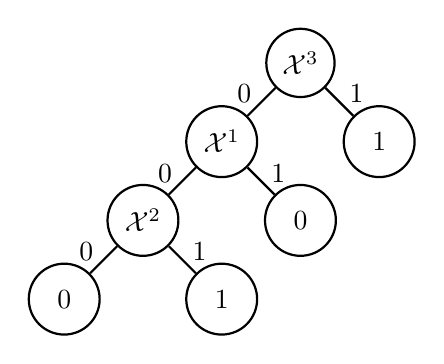
\begin{tikzpicture}
	\node[draw,thick,circle] at (3,3) (a) {$\mathcal{X}^3$};
	\node[draw,thick,circle,minimum size=0.9cm] at (2,2) (b) {$\mathcal{X}^1$};
	\node[draw,thick,circle,minimum size=0.9cm] at (4,2) (c) {$1$};
	\draw[thick] (a) -- (b) node[midway,left ,yshift=.1cm] {$0$};
	\draw[thick] (a) -- (c) node[midway,right,yshift=.1cm] {$1$};
	\node[draw,thick,circle,minimum size=0.9cm] at (1,1) (d) {$\mathcal{X}^2$};
	\node[draw,thick,circle,minimum size=0.9cm] at (3,1) (e) {$0$};
	\draw[thick] (b) -- (d) node[midway,left ,yshift=.1cm] {$0$};
	\draw[thick] (b) -- (e) node[midway,right,yshift=.1cm] {$1$};
	\node[draw,thick,circle,minimum size=0.9cm] at (0,0) (f) {$0$};
	\node[draw,thick,circle,minimum size=0.9cm] at (2,0) (g) {$1$};
	\draw[thick] (d) -- (f) node[midway,left ,yshift=.1cm] {$0$};
	\draw[thick] (d) -- (g) node[midway,right,yshift=.1cm] {$1$};
  \end{tikzpicture}
  \end{center}
  \begin{itemize}
    \item {\color{red} $S=\{(0,0,0,0),(0,1,0,1),(1,0,1,1),(1,1,0,0)\}$}
  \end{itemize}
\end{frame}

\begin{frame}
  \frametitle{Support vector machines}
  \begin{itemize}
	\item Derive the dual optimization problem for SVMs
  \end{itemize}
\end{frame}

\begin{frame}
  \frametitle{Support vector machines}
  \begin{itemize}
  \item The constrained optimization problem is given by
  \begin{align*}
	\min_{w,b} \;\; & \frac 1 2 \langle w, w \rangle\\
	\mathrm{s.t.} \;\; & y_i(\langle w, x_i\rangle + b) \geq 1, \;\; \forall i\in[m]
  \end{align*}
  \pause
  \item The Lagrangian is given by
  \[\mathcal{L}(w,b,\alpha) = \frac 1 2 \langle w, w \rangle + \sum_{i=1}^m \alpha_i (1 - y_i(\langle w, x_i\rangle + b))\]
  \end{itemize}
\end{frame}

\begin{frame}
  \frametitle{Support vector machines}
  \begin{itemize}
  \item The Lagrangian is given by
  \[\mathcal{L}(w,b,\alpha) = \frac 1 2 \langle w, w \rangle + \sum_{i=1}^m \alpha_i (1 - y_i(\langle w, x_i\rangle + b))\]
  \pause
  \item The KKT conditions are given by
  \begin{align*}
	\nabla\mathcal{L}(w,b,\alpha) &= 0\\
	\alpha_i (1 - y_i(\langle w, x_i\rangle + b)) &= 0, \;\; \forall i\in[m]
  \end{align*}
  \end{itemize}
\end{frame}

\begin{frame}
  \frametitle{Support vector machines}
  \begin{itemize}
  \item Setting the gradient of the Lagrangian to 0 yields
  \[
	\nabla\mathcal{L}(w,b,\alpha) =
	\left(
	\begin{array}{c}
		\frac {\partial\mathcal{L}(w,b,\alpha)} {\partial w_1}\\
		\vdots \\
		\frac {\partial\mathcal{L}(w,b,\alpha)} {\partial w_d}\\[4pt]
		\frac {\partial\mathcal{L}(w,b,\alpha)} {\partial b}
	\end{array}
	\right) =
	\left(
	\begin{array}{c}
		w_1 - \sum_{i=1}^m \alpha_i y_i x_i^1\\
		\vdots \\
		w_d - \sum_{i=1}^m \alpha_i y_i x_i^d\\[4pt]
		- \sum_{i=1}^m \alpha_i y_i
	\end{array}
	\right) = 0
  \]
  \pause
  \item Solution given by $w^* = \sum_{i=1}^m \alpha_i y_i x_i$ and $\sum_{i=1}^m \alpha_i y_i = 0$
  \pause
  \item For any {\color{red} $k\in[m]$} such that {\color{red} $\alpha_k>0$} we have {\color{red} $1 = y_k(\langle w,x_k\rangle + b^*)$}
  \begin{align*}
	\Leftrightarrow \;\; y_k &= {\color{blue} y_k^2} (\langle w, x_k \rangle + b^*) = \langle w, x_k \rangle + b^*\\
	\Leftrightarrow \;\; b^* &= y_k - \langle w, x_k \rangle
  \end{align*}
  \end{itemize}
\end{frame}

\begin{frame}
  \frametitle{Support vector machines}
  \begin{itemize}
  \item Inserting $w^*$ and $b^*$ into the Lagrangian yields the dual objective
  \begin{align*}
	g(\alpha) &= \mathcal{L}(w^*,b^*,\alpha) = \frac 1 2 \langle \sum_{i=1}^m \alpha_i y_i x_i, \sum_{j=1}^m \alpha_j y_j x_j \rangle + \sum_{i=1}^m \alpha_i\\
	 & \hspace*{2.35cm} - \sum_{i=1}^m \alpha_i y_i \langle \sum_{j=1}^m \alpha_j y_j x_j, x_i\rangle - b^* {\color{red} \sum_{i=1}^m \alpha_i y_i}\\
	 &= \sum_{i=1}^m \alpha_i - \frac 1 2 \sum_{i=1}^m \sum_{j=1}^m \alpha_i \alpha_j y_i y_j \langle x_i, x_j \rangle + {\color{red} 0}
  \end{align*}
  \end{itemize}
\end{frame}

\begin{frame}
  \frametitle{Support vector machines}
  \begin{itemize}
  \item The dual optimization problem is given by
  \begin{align*}
	\max_\alpha \;\; & \sum_{i=1}^m \alpha_i - \frac 1 2 \sum_{i=1}^m \sum_{j=1}^m \alpha_i \alpha_j y_i y_j \langle x_i, x_j \rangle\\
	\mathrm{s.t.} \;\; & \alpha_i \geq 0, \;\; \forall i\in[m]\\
	& \sum_{i=1}^m \alpha_i y_i = 0
  \end{align*}
  \end{itemize}
\end{frame}

\end{document}

